基于机器视觉的人体运动类型识别

摘要

本文提出用基于深度训练的机器视觉模型,在只使用由 Kinect
采集回来的人体骨架的运动数据的条件下进行人体运动类型的识别。使用由
Kinect
采集回来骨架模型是因为它具有数据容易获取,数据维度少的特点,可以方便存储、传输。而文章中的这个识别模型在训练时除了
CAD-60
数据集提供的人体骨架数据,没有使用任何的先验知识来进行人体运动类型的识别。这样子可以减少在数据的预处理阶段中人工的干预,只由机器自己来进行特征的提取,这样子可以减少人工提取特征时出现的错误。这也能使最终的模型的泛化性更优秀,鲁棒性更好。从而让模型对人体运动类型有更好的理解与识别。模型上,本文测试了卷积神经网络、自编码器、降噪自编码器、限制玻耳兹曼机以及混合的多种结构,并实验了多种网络训练上的用来加强效果的算法,比如一些正规化的方法和其他新的激活函数,最后选择了卷积神经网络作为自动特征提取的模型,并在其后面配合上多层感知机来进行分类。\textbackslash{}关键字:人体运动类型识别,CAD-60
数据集,深度训练,卷积神经网络,自编码器,限制玻耳兹曼机,Kinect

HUMAN ACTION RECOGNITION BASE ON COMPUTER VISION

Abstract

We propose in the paper a computer vision model base on deep learning,
which can recognize the human action only base on the data source in the
skeletons of the human from Kinect. Using the skeletons from Kinect is
because it is easy to get, to store and to transfer, and it has the less
order of the data. This model only use the human skeletons data from the
CAD-60 dataset to recognize the human action without using any prior
knowledge. It can reduce the works from the human on the stage of
preprocessing and hand the feature extraction to the computer, which can
reduce the error from the human-engineer. It can also improve
generalization performance and robustness of the model, And give the a
understanding of the human action. In the paper, we do the experiment on
with convolutional neural networks, autoencoder, denoising autoencoder,
Restricted Boltzmann Machines and the some of their mixture, and it also
do some experiments for the tricks which can improve the nerual network,
such as some regularization methods or other activation functions. In
the end, we choose the convolutional neural networks for the feature
extraction. And use the multilayer perceptron as the follow
classifier.\textbackslash{}keywords: Human action recognition, CAD-60
dataset, deep models, convolutional neural networks, autoencoder,
Restricted Boltzmann Machines, Kinect

\section{绪论}\label{ux7eeaux8bba}

\subsection{引言}\label{ux5f15ux8a00}

计算机自动去理解人类的行为、动作还有跟环境之间的交流互动,在近年来逐渐地成为了一个热门的领域,因为这个技术在很多领域都有可以使用的地方。比如现代社会快速的生活节奏和巨大的工作压力,严重影响着个人的身体健康。科学的运动可以提高身体素质增强运动能力,进而降低患病的风险(尤其是一些慢性疾病),例如糖尿病、血脂异常、高血压等。而进行科学运动的前提是实现人体运动类型的准确识别。
在信息安全领域,通过智能监控的方式利用计算机自动对视频中人体的运动类型进行识别从而为监控或者案件侦破提供依据也具有着重要的意义和广泛的用途。
在人机交互领域可以通过手势、身体姿态等信息对除了辅助交互输入设备以及自然语言分析进行补充,提高计算机和人进行交互的能力,使之更有趣。
在大型的图像数据库或者互联网上的信息中还可以利用人体运动类型的识别,对部分信息进行标注和理解,进而提供搜索和训练的能力。
本课题的任务是通过使用深度训练的相关理论,尝试构造用基于深度训练的机器视觉模型,应用于人体运动类型的识别,从而让模型对人体运动类型有更好的理解与识别。

\subsection{人体运动类型识别的相关研究现状}\label{ux4ebaux4f53ux8fd0ux52a8ux7c7bux578bux8bc6ux522bux7684ux76f8ux5173ux7814ux7a76ux73b0ux72b6}

\subsubsection{人体运动数据源的获得}\label{ux4ebaux4f53ux8fd0ux52a8ux6570ux636eux6e90ux7684ux83b7ux5f97}

首先,对于人体运动识别的数据的来源存在着几种不同的种类\{{[}\}1\{{]}\}。例如由
RGB
摄像机、距离传感器或其他遥感的方式。使用深度传感器来进行人体运动识别的发展始于
80
年代初。过去的研究主要集中在训练和认识到从视频序列(可见光相机)所采集的数据中。可见光视频的主要问题是从单目视频传感器捕捉得到的人体运动存在相当大的损失。由于视频天生的对的人体行为识别的限制,尽管已经有了过去几十年的努力,但通过视频来识别人体运动,仍然是非常具有挑战性的。
而得益于近期发布的成本低廉的深度传感器,我看到了和 3D
数据相关的研究越来越多了。从过去的 20 年里,我获得 3D
数据的方法,一共分为三类。一种方法是通过使用基于标记的动作捕捉系统,如
MoCap。 第二种方式是通过立体视觉: 从多个角度捕获 2D
图像序列,通过从多个视图来重建三维信息。第三种方式是使用距离传感器(使用类似
TOF
原理的传感器)。深度相机在过去几年里取得迅速的发展。最近出现的深度照相机可以在相对低廉的成本和较小的尺寸里给我提供较高的帧率和分辨率,这导致出现了许多新的研究中的动作识别都是采用的三维数据。

\subsubsection{人体动作识别的主要问题}\label{ux4ebaux4f53ux52a8ux4f5cux8bc6ux522bux7684ux4e3bux8981ux95eeux9898}

基于视觉的人体动作识别里有四个主要的问题。第一个问题的挑战性比较小
\{{[}\}2\{{]}\} \{{[}\}3\{{]}\}:闭塞、 杂乱的背景、
阴影和不同光照条件会让运动难以分割或者被错误地识别。这是从 RGB
视频行为识别的一大难点。引入 3D
数据可以在很大程度上通过提供现场的结构信息,从而缓解这个问题。第二个是视角的变换\{{[}\}2\{{]}\}
\{{[}\}4\{{]}\} \{{[}\}5\{{]}\} 和
\{{[}\}6\{{]}\}。相同的操作可以从不同的角度产生不同的``外观''。传统的
RGB
相机解决这一问题的方法主要是引入多个同步的摄像机,同时获得多个视角的图像,但对于某些应用程序,这不是件容易的事。不过对于三维运动捕捉系统,这不是一个严重的问题。而如果通过深度图像来进行识别的话,这个问题也会有部分被缓解,因为从轻微旋转的视角的外观可以推断深度的信息。这一点并不完全解决问题,因为摄像机始终还只是在对象的一侧上,这个距离图像只提供了部分的信息,还是没有人知道这个对象的另一面是什么样子的。如果可以运用单一深度相机来精确地推断出人的骨架模型,则可以通过骨架模型的信息来构造一种视图不变识别的算法。第三个问题是放缩上的差异,因为人离相机的距离的不同会影响主体的大小从而影响运动的识别。而在
RGB 视频中,这可以通过在多个尺度下的\{{[}\}7\{{]}\}
特征提取解决了。而在深度视频中,这可以很容易调整,因为真正的主体的 3D
尺寸直接是已知的。第四个问题是同一种类内的变异性和不同种类之间的相似性问题\{{[}\}8\{{]}\}。人可以通过不同的身体部位在不同的方向上做动作,但不同的方向和两个动作仅只有只由非常细微的细节来区分。而这个不管对于使用哪种数据的来源的算法来说都仍然是一个非常困难的问题。\textbackslash{}前三个问题基本上都可以通过使用三维空间上的图像或者类似骨架之类的模型来解决,所以本文使用的数据来源是由传感器采集计算直接得到的骨架数据。

\subsubsection{人体动作识别的相关研究成果}\label{ux4ebaux4f53ux52a8ux4f5cux8bc6ux522bux7684ux76f8ux5173ux7814ux7a76ux6210ux679c}

从各种论文来看,相关研究的重点都是集中在寻找合适的特征,如时空趣点特征STIP\{{[}\}9\{{]}\}、骨架模型\{{[}\}9\{{]}\}\{{[}\}10\{{]}\}\{{[}\}11\{{]}\}、方向梯度直方图(HOG:Histogram
of oriented gradients)\{{[}\}12\{{]}\}\{{[}\}13\{{]}\} 、
光流场方向直方图(HOF:Histograms of Optical
Flow)\{{[}\}12\{{]}\}\{{[}\}14\{{]}\}\{{[}\}15\{{]}\}、EigenJoints\{{[}\}16\{{]}\}等特征或者是它们的一些拓展和变形,如方向HOF\{{[}\}17\{{]}\},以及根据这些特征进行进一步的组合来产生更高级的特征。\textbackslash{}然后把这些特征通过分类器如贝叶斯模型\{{[}\}16\{{]}\}\{{[}\}18\{{]}\}、k近邻kNN\{{[}\}19\{{]}\}、支持向量机
SVM\{{[}\}12\{{]}\}\{{[}\}19\{{]}\}\{{[}\}20\{{]}\}\{{[}\}14\{{]}\}\{{[}\}21\{{]}\}\{{[}\}22\{{]}\}、隐马尔可夫模型
HMM\{{[}\}19\{{]}\}\{{[}\}11\{{]}\}来进行有监督的训练得到分类。分类器之间也可以通过串联\{{[}\}16\{{]}\}或者并联(票决、加权)来加强分类的效果。

\subsubsection{使用深度训练进行有效的特征提取}\label{ux4f7fux7528ux6df1ux5ea6ux8badux7ec3ux8fdbux884cux6709ux6548ux7684ux7279ux5f81ux63d0ux53d6}

上一节所说到的特征的选取或者是计算一般是通过人工方式得到的。而这种人工方式得到的特征对应用的领域有较强的依赖性,也就是说,换一个研究的问题之后可能同样的特征就不能再适用了。\textbackslash{}而深度训练\{{[}\}23\{{]}\}的提出,某种程度上解决了这些关于特征提取的这些问题。
模仿出人脑表征信息的高效和鲁棒性一直是近几十年来人工智能研究中的一个核心。而人类不仅每时每刻都暴露在由感官接收的无数的数据中,而且还能够通过某些方法捕捉到这些数据关键的部分来让自己能够以简单的方式在未来使用。早在五十年前,提出了动态规划理论以及开创了最优化控制领域的
Richard Bellman
就曾断言,数据的高维度是在人工智能科学和工程应用中的根本障碍。其中主要的困难,尤其是在模式分类的应用中,就是数据训练的难度会随着数据维度的线性增长,发生指数级的增长\{{[}\}24\{{]}\}。而克服这个问题的主流方法就是以一定的方式(比如分类器、SIFT
算法)对数据进行预处理来减少数据的维度,这样数据就可以被有效地处理。这种减少维度的做法一般被称为特征提取。因此,可以认为,在很多模式识别系统的背后的智能其实被转移到了人工的特征提取处理上去了,而这种人工的做法有时会很困难而且会高度依赖于具体的应用场景\{{[}\}25\{{]}\}。此外,如果不完整或者错误的特征被提取出来了,那么分类处理的性能就会从根本上受到限制。
最近,神经科学在哺乳类动物大脑上的新发现告诉我,我可以通过一个复杂的深层网络结构来对数据自动地进行预处理。这就是深度训练的基本来源。

\section{模型原理}\label{ux6a21ux578bux539fux7406}

\subsection{特征提取}\label{ux7279ux5f81ux63d0ux53d6}

得益于 Microsoft Kinect 的发布,通过它采集、处理 RGB-D
图像并提取出人体骨架模型的做法已经非常的流行,而且它也能有效地对原数据进行了第一步的特征提取,所以本文的算法是基于由
Kinect
采集出来的人体骨架数据来进行研究的。\textbackslash{}在这一章里,我先是总结了几种特征提取的模式,然后主要阐述了一些用来对原数据进行非人工的特征提取的方法,并对各种方式进行了实验,列出了对比的数据,最终选择了卷积神经网络来进行特征的自动提取。

\subsubsection{特征提取模式}\label{ux7279ux5f81ux63d0ux53d6ux6a21ux5f0f}

\paragraph{人工特征提取}\label{ux4ebaux5de5ux7279ux5f81ux63d0ux53d6}

这种模式是指是使用一些人工设计的,由人对源数据的理解所构造的算法来进行特征提取如之前说过的骨架模型、时空特征点之类的方法。也就是在识别的模型里加入一些人对数据的理解的先验的知识来加强模型的效果。这种方式会随着不同的数据或者不同的应用领域而改变,每换一个领域可能都需要使用人的知识和能力来进行训练、归纳和总结,然后选择一个特征提取的方式,如下图所示

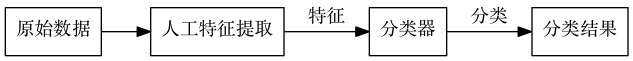
\includegraphics{picture/learning-framework1.png} 图1.人工特征提取

\paragraph{无监督训练特征提取}\label{ux65e0ux76d1ux7763ux8badux7ec3ux7279ux5f81ux63d0ux53d6}

这个类型主要是使用无监督训练的方法如限制玻耳兹曼机
RBM,自编码器,或者一些类似主要成分分析 PCA
的算法,在不需要数据集带有标签的前提下能够对数据的特征进行提取,发现特征内在的信息,从而减少数据的冗余,减少数据的维度。而这类型的模式如下图所示\textbackslash{}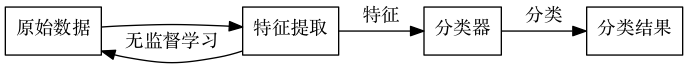
\includegraphics{picture/learning-framework2.png}
图2.无监督特征提取

\paragraph{有监督特征提取}\label{ux6709ux76d1ux7763ux7279ux5f81ux63d0ux53d6}

这个类型是使用有监督训练的方法,在特征提取里面把标签的信息也考虑进去,从而使特征提取的结果更有针对性,对后面的分类更有利,这类型里的算法有
CNN
卷积神经网络,过程则如下图所示\textbackslash{}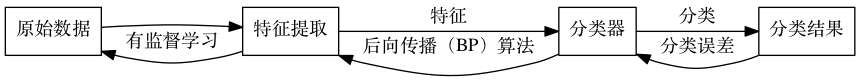
\includegraphics{picture/learning-framework3.png}\textbackslash{}图3.有监督特征提取

\subsubsection{特征提取模型}\label{ux7279ux5f81ux63d0ux53d6ux6a21ux578b}

\paragraph{主要成分分析
PCA}\label{ux4e3bux8981ux6210ux5206ux5206ux6790-pca}

主要成分分析\{{[}\}26\{{]}\}\{{[}\}27\{{]}\}
里的假设是,在数据里变化最大的那些因素就是最有价值的因素,因此,只要把输入的数据的空间找到一个变换,这个变换可以把数据里变化最大的因素提取出来,其他变化不那么大(利用价值比较小)的舍弃不看,就可以降低数据的维度,从而减少后面的计算的难度了。\textbackslash{}首先要做的是数据的预处理,也就是数据的均值中心化和方差归一化:\textbackslash{}1.数据的均值中心化,也就是把数值变化范围的中心移至
0 处:\textbackslash{}{[} x\^{}\{(i)\} = x\^{}\{(i)\} - \mu =
x\^{}\{(i)\} - \frac{1}{m} \sum\_\{i=1\}\^{}m \{x\^{}\{(i)\}\}{]}
2.数据的方差归一化:\textbackslash{}{[} x\_j\^{}\{(i)\} = x\_j\^{}\{(i)\}
/ \sigma\_j = x\_j\^{}\{(i)\} /
\sqrt{\frac{1}{m} \sum_{i=1}^m {(x_{j}^{(i)})^2}} {]}

然后进行 PCA 核心环节:\textbackslash{}1.首先求协方差矩阵: {[}\sum =
\frac{1}{m}
\sum\_\{i=1\}\textsuperscript{\{m\}(x}\{(i)\})(x\textsuperscript{\{(i)\})}T{]}
2.求得协方差矩阵的特征向量(U)并按特征值(\lambda\_n)从大到小依次排列得到:\textbackslash{}{[}U={[}u\_1
u\_2 \ldots{}. u\_n{]}{]} 3.按照一定的方法取 (k)
,比如一个常见的经验法则是选择 (k) 以保留99\%的方差:
{[}\frac{\sum^{k}_{j=1}\lambda_j}{\sum^{n}_{j=1}\lambda_j}
\textgreater{}= 0.99{]}\textbackslash{}4.取前 (k)
个特征值对应的特征向量,组成新的特征向量矩阵(U')。并与 (x)
相乘,得到新的降维后的数据 (x'):\textbackslash{}{[}U' = {[}u\_1 u\_2
\ldots{}. u\_k{]}{]} {[}x' = U'\^{}T * x{]}

\paragraph{自编码器
Autoencoders}\label{ux81eaux7f16ux7801ux5668-autoencoders}

一个自编码器\{{[}\}28\{{]}\}\{{[}\}29\{{]}\}会对一个输入 (x∈{[}0,
1{]}\^{}\{d\}) 经过一次线性变换之后得到一个确定的表达
(y∈{[}0,1{]}\^{}\{d′\}) :\textbackslash{}{[}y = s(Wx +
b){]}\textbackslash{}这其中的 (s) 是非线性环节,比如 sigmoid
函数。然后,这个潜在的对输入的表达 (y)
(或者说编码),会被再一次地重新映射(或者说解码)到一个和 (x)
一样结构大小的重建出来的
(z)。(上述的式子没有使用矩阵变换的形式)。这里的 (z) 应该视为在 (y)
的表达下的 (x) 的一种预测。而重建的里面的 (W') 可以限制为正向映射的 (W)
的倒置:(W'=W\^{}T)。而这个模型的参数(比如
(W',b,b'))可以通过使平均重建误差最小化来进行优化。\textbackslash{}重建误差可以通过很多方法进行测量,这个依赖于编码的输入的分布。传统的\textbackslash{}{[}L(xz)
=
\textbar{}\textbar{}x-z\textbar{}\textbar{}\^{}2{]}\textbackslash{}也是可以使用的。\textbackslash{}这里面的
(y)
是输入的数据的空间中的主要因子的一个表达。这个跟主要成分分析中的捕捉输入数据空间的主要因子非常类似。而事实上,如果中间的隐含层(编码)是一个线性变换而且是使用均方误差来训练网络的话,有
(k) 个隐含单元就意味着其实是在找出原数据的前 (k)
主要成分。但是如果隐含层是非线性的话,自编码器就跟 PCA
很不一样了,因为它还具备了捕捉输入数据里多模态的部分。

\paragraph{卷积神经网络}\label{ux5377ux79efux795eux7ecfux7f51ux7edc}

卷积神经网络 CNNs
\{{[}\}30\{{]}\}\{{[}\}31\{{]}\}是一个专门为二维数据(例如图片和视频)设计的多层神经网络的系列。
CNNs
是第一种真正意义上成功的深度训练方法,它能够成功地用一种鲁棒的方式训练出多层的神经网络。相比起普通的多层神经网络,卷积神经网络有很多独有的特点。

\subparagraph{稀疏连接}\label{ux7a00ux758fux8fdeux63a5}

卷积神经网络利用了空间的局部相关性,相邻两层之间只进行了局部的连接,而不是像多层感知机
MLP 一样使用全连接的方式。换句话说,隐层 m 的单元的输入来自于层 m-1
在空间上连续的感受野的单位的一个子集。具体的如下图所示:\textbackslash{}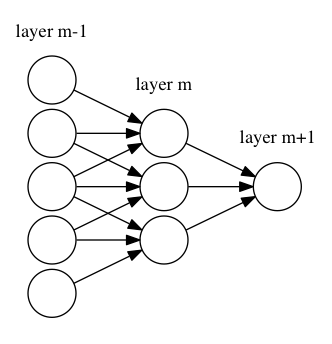
\includegraphics{picture/sparse-connectivity.png}\textbackslash{}图4.稀疏连接

想象一下,层 m-1 是输入,而在上面的图中,层 m 的单位感受野宽度为 3
,因此层 m 的每个神经元只连接到输入层的 3 个相邻的神经元。在层 m+1
中也有与下方图层类似的连接性。我说他们的感受野宽度也是
3,但实际上他们相对于输入的层 m-1 的感受野的是 5。就是说每个 层m
里的单元都会响应在其关于视网膜的感受野的变化。这个层级结构确保了训练出来的
filter
可以对来自于局部空间的输入产生最强烈的反应。因此,也正如上面所说的,叠加这种层级的结构会导致(非线性)的
filter,可以使它越到后面的层,响应对应的输入感受野更大。例如,在隐藏图层
m + 1 单元可以编码 5 宽度 (以像素的空间)
的非线性特征。\textbackslash{}这种连接的编码方式,比起普通的全连接的神经网络显然可以有效地减少连接的数量,从而能容纳更多的层数,对输入的数据进行更复杂的描述,加强了模型的表达能力。而且,只与上一层的相邻的局部的几个神经元连接的方式,可以使模型具备一定程度的某维度维度上的不变性。

\subparagraph{共享权值}\label{ux5171ux4eabux6743ux503c}

除了稀疏连接之外,每一个 filter
都是一套参数应用在整个输入空间上的。具体如图所示,\textbackslash{}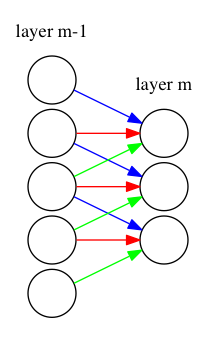
\includegraphics{picture/shared-weights.png}\textbackslash{}图5.权值共享\textbackslash{}红色、蓝色、绿色三种线代表三个权值(W、b,即权值和偏置),层
m
中每个单元都是由相同的这个三个权值和他们对应的感受野里的输入神经元计算出来的。假如没有权值共享,则需要的权值就有
(3 * 3 = 9)
个,由此可见,权值共享使得需要进行优化的参数大大地减少了,使得我能够更有效地进行特征提取。通过控制模型的规模,卷积网络对视觉问题的泛化能力非常好。

\subparagraph{池化(pooling)}\label{ux6c60ux5316pooling}

以上两个特点都是由通过使用卷积核卷积计算生成多个特征图的方式实现的。而完整的卷积神经网络的结构里,还有池化的层用来进行二次的采样,比如使用一个
(N*N)
的求最大值窗口或者平均值窗口进行降采样。这种操作被称为池化,池化的操作的作用是可以提供一定的空间位移的不变性以及进一步减少数据的维度,一般池化之后会通过一个激活函数得到一个新的网络的层。

\subparagraph{完整模型}\label{ux5b8cux6574ux6a21ux578b}

以上两个特点都是由通过使用卷积核卷积计算生成多个特征图的方式实现的。而完整的卷积神经网络的结构里,还有其他的东西,以
LeNet为例,展示一下完整的卷积神经网络的结构。\textbackslash{}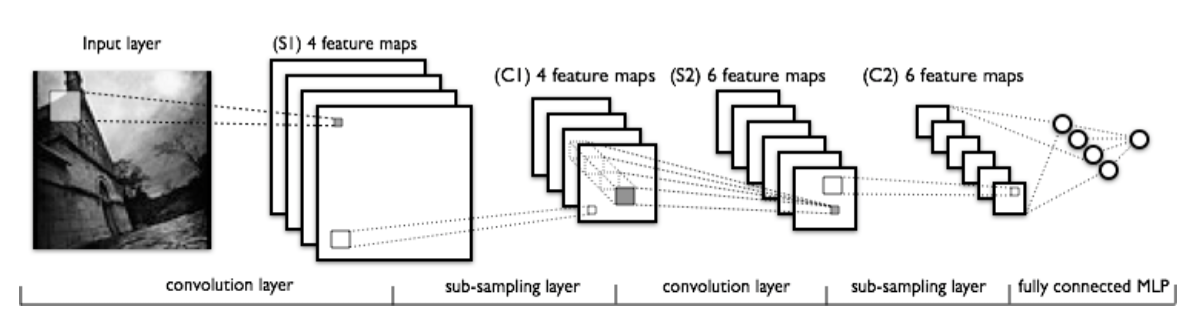
\includegraphics{picture/lenet.png}\textbackslash{}图6.LeNet-网路\textbackslash{}上图中的网络输入图像通过
4 个可训练的滤波器和偏置在 S1 的位置产生了 4
个特征图。特征图中的每个图通过池化并通过一个激活函数之后得到一个 C1
位置上的 4 个新的特征图。然后会通过一个新的卷积层然后得到新的 6 个特征图
S2。这些将再一次池化得到
C2。最终这些像素的值进行光栅化、摊平成一个向量,这个向量就是这个网络里提取得到的特征。这些特征之后就可以输入到一个常规的分类器里,比如神经网络(多层感知机
MLP)里,最终由这个分类器进行分类结果的计算和输出。\textbackslash{}而这些卷积核的权值和偏置,还有其他用到的权值则使用后向传播算法来进行计算出梯度,然后通过梯度下降法之类的算法进行优化,从而训练出来一个有效的特征提取的卷积神经网络。

\subsection{多层感知机(MLP)}\label{ux591aux5c42ux611fux77e5ux673amlp}

特征提取完了之后,需要把特征交到后面的分类器进行分类,而由于有监督的特征提取网络需要得到分类错误后的传递过来的误差,所以需要需要使用可以进行后向传播的分类器,这里面比较经典的分类器就是多层感知机(MLP)也就是普通的神经网络\{{[}\}32\{{]}\}。

神经网路由神经元组成:\textbackslash{}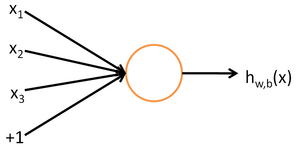
\includegraphics{picture/single-neuron.png}\textbackslash{}图7.典型神经网络中的神经元\textbackslash{}上图中的神经元实际上是一个以
(x\_1, x\_2, x\_3) 及截距 (+1) 为输入值的运算单元,其输出为
(h\_\{W,b\}(x) = f(W\^{}Tx) = f(\sum\emph{\{i=1\}\^{}3 W}\{i\}x\_i +b))
,其中函数 (f)
被称为``激活函数''。激活函数的作用主要是为神经网络引入非线性环节,使其对非线性的函数具有更好的拟合能力。一般我会选用
sigmoid 函数作为激活函数:\textbackslash{}{[}f(z) =
\frac{1}{1+\exp(-z)}{]}

典型的神经网络如图所示:\textbackslash{}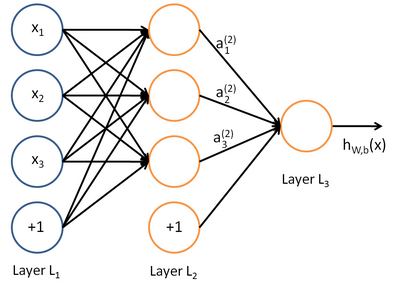
\includegraphics{picture/MLP.png}\textbackslash{}图8.典型多层神经网网络\textbackslash{}如上图所示,把多个神经元按上图的形式以多层的形式串联起来,就可以得到可以一个神经网络用来对数据进行训练、拟合或者分类。

\subsubsection{前向传播}\label{ux524dux5411ux4f20ux64ad}

输入的值经过一层一层的神经元的计算、激活,一直到达最后一层,并得到值称之为前向传播,对于图
8 中的模型,前向传播的计算步骤如下所示:\textbackslash{}{[}
a\_1\^{}\{(2)\} = f(W\_\{11\}\^{}\{(1)\}x\_1 + W\_\{12\}\^{}\{(1)\} x\_2
+ W\_\{13\}\^{}\{(1)\} x\_3 + b\_1\^{}\{(1)\}){]} {[} a\_2\^{}\{(2)\} =
f(W\_\{21\}\^{}\{(1)\}x\_1 + W\_\{22\}\^{}\{(1)\} x\_2 +
W\_\{23\}\^{}\{(1)\} x\_3 + b\_2\^{}\{(1)\}){]} {[} a\_3\^{}\{(2)\} =
f(W\_\{31\}\^{}\{(1)\}x\_1 + W\_\{32\}\^{}\{(1)\} x\_2 +
W\_\{33\}\^{}\{(1)\} x\_3 + b\_3\^{}\{(1)\}){]} {[} h\_\{W,b\}(x) =
a\_1\^{}\{(3)\} = f(W\_\{11\}\textsuperscript{\{(2)\}a\_1}\{(2)\} +
W\_\{12\}\^{}\{(2)\} a\_2\^{}\{(2)\} + W\_\{13\}\^{}\{(2)\}
a\_3\^{}\{(2)\} + b\_1\^{}\{(2)\}{]}\textbackslash{}如果把权值 W
表示为矩阵,且将激活函数 (f())
扩展为使用向量则上列等式可以更加简洁地表示为:\textbackslash{}{[}z\^{}\{(2)\}
= W\^{}\{(1)\}x + b\textsuperscript{\{(1)\}{]} {[}a}\{(2)\} =
f(z\^{}\{(2)\}){]} {[}z\^{}\{(3)\} = W\^{}\{(2)\} a\^{}\{(2)\} +
b\^{}\{(2)\}{]} {[}h\_\{W,b\}(x) = a\^{}\{(3)\} = f(z\^{}\{(3)\}){]}

\subsubsection{后向传播}\label{ux540eux5411ux4f20ux64ad}

上述的前向传递是根据输入,通过网络逐层计算出来合适的结果,但是网络的里的权值、偏置需要确定,所以可以通过梯度下降法来进行对这些参数,也就是对神经网络进行求解。而对于单个输入的测试样例
((x,y)),其代价函数为: {[}J(W,b; x,y) = \frac{1}{2}
\textbar{}\textbar{} h\_\{W,b\}(x) - y
\textbar{}\textbar{}\^{}2{]}\textbackslash{}只要得到每一个参数的关于代价函数的偏导数,我就可以使用梯度下降法来进行优化。\textbackslash{}而求解每一个参数的偏导数就需要使用反向传播算法了。\textbackslash{}反向传播算法的思路如下:给定一个样例
((x,y)),我首先进行\texttt{前向传播\textquotesingle{}\textquotesingle{}运算,计算出网络中所有的激活值,包括\ \textbackslash{}(h\_\{W,b\}(x)\textbackslash{})\ 的输出值。之后,针对第\ \textbackslash{}(l\textbackslash{})\ 层的每一个节点\ \textbackslash{}(i\textbackslash{}),我计算出其}残差''
(\delta\^{}\{(l)\}\_i)
,该残差表明了该节点对最终输出值的残差产生了多少影响。对于最终的输出节点,我可以直接算出网络产生的激活值与实际值之间的差距,我将这个差距定义为
(\delta\^{}\{(n\_l)\}\_i) (第 (n\_l)
层表示输出层)。对于隐藏单元我将基于节点(第 (l+1)
层节点)残差的加权平均值计算 (\delta\^{}\{(l)\}\_i) ,这些节点以
(a\^{}\{(l)\}\emph{i)
作为输入。\textbackslash{}后向传播算法可以具体表示为以下步骤:\textbackslash{}1.进行前馈传导计算,利用前向传导公式,得到
(L\_2, L\_3, \ldots) 直到输出层 (L}\{n\_l\})
的激活值。\textbackslash{}2.对输出层(第 (n\_l) 层),计算:
{[}\delta\^{}\{(n\_l)\} = - (y - a\^{}\{(n\_l)\})
\bullet f'(z\^{}\{(n\_l)\}){]} 3.对于 (l=n\_l-1, n\_l-2, n\_l-3, \ldots,
2) 的各层,计算: {[}\delta\^{}\{(l)\} =
\left((W\textsuperscript{\{(l)\})}T \delta\^{}\{(l+1)\}\right)
\bullet f'(z\textsuperscript{\{(l)\}){]} 4.计算最终需要的偏导数值:
{[}\nabla\emph{\{W\^{}\{(l)\}\} J(W,b;x,y) =
\delta\textsuperscript{\{(l+1)\}(a}\{(l)\})\^{}T,{]}
{[}\nabla}\{b}\{(l)\}\} J(W,b;x,y) = \delta\^{}\{(l+1)\}.{]}

\section{实验}\label{ux5b9eux9a8c}

本章中,首先会介绍一些我在实验过程中使用的一些能够增强模型效果、速度、泛化能力的技巧,然后会结合编程实践给出一些编程框架的对比,以及不同算法下的准确率的比较。

\subsection{神经网络使用技巧}\label{ux795eux7ecfux7f51ux7edcux4f7fux7528ux6280ux5de7}

\subsubsection{数据、网络预处理{[}33{]}}\label{ux6570ux636eux7f51ux7edcux9884ux5904ux7406lecun2012}

\paragraph{对输入数据进行标准化}\label{ux5bf9ux8f93ux5165ux6570ux636eux8fdbux884cux6807ux51c6ux5316}

由于训练率对于每一个参数都是一样的,所以为了加快收敛,可以让所有参数都以相同的标准进行线性变换,映射到一个一致的范围里对输入的。具体的变换要求如下:\textbackslash{}A、训练集的每个输入变量的均值要接近于0;\textbackslash{}B、对输入变量进行缩放,使他们的方差具有相同的值;\textbackslash{}C、输入变量最好是不相关的。\textbackslash{}如图所示:\textbackslash{}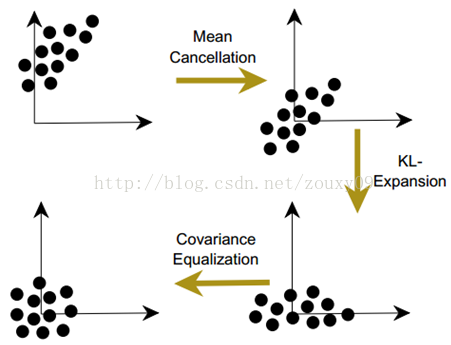
\includegraphics{picture/normalizing-the-inputs.png}\textbackslash{}图9.输入标准化

\paragraph{参数的初始化}\label{ux53c2ux6570ux7684ux521dux59cbux5316}

参数的初始值对训练过程有着重大的影响。我对参数初始化的原则是:参数应该随机初始化在能让
sigmoid
函数在线性区域激活的值。如果参数全部都很大,那sigmoid一开始就饱和了,这样就会得到一个非常小的梯度值,那参数更新就会很慢,训练也会很慢。使
sigmoid 函数工作在线性区域激活除了需要输入数据标准化到其标准差为
1,还需要参数初始值,也就是连接神经元的权值的初始值的标准差也能为
1。最简单的做法就是,给参数初始化的时候使用正态分布采样得到,那么参数就会均值为零,且方差近似1。

\paragraph{打乱样本的训练顺序}\label{ux6253ux4e71ux6837ux672cux7684ux8badux7ec3ux987aux5e8f}

在使用后向传播算法进行训练的时候,有一个原则是使用意料之外的样本来训练,收敛得会更快。一般来说,训练用的数据都会是规整的,按顺序排列的,比如我使用的数据集里,人体的运动都是按照时间顺序在一个大的视频里分别进行切片的,所以相邻的训练数据有很大可能是来自于同一个类型甚至是同一个视频的。而这一节的这个技巧就是在粗糙地选择来自不同类的样本,也就是说,尽量让每一次的训练采用的样本都来自不一样的类型,最简单的做法就是把样本的顺序打乱。因为同一个类的训练样本很大可能携带的是相似的信息,而相似的信息很有可能让网络落入一个局部的最优解处。所以为了提高模型的泛化性能,每次使用来进行训练的样本最好是随机地而不是按照顺序地进行选择。

\subsection{网络设计技巧}\label{ux7f51ux7edcux8bbeux8ba1ux6280ux5de7}

\subsubsection{加入正规化环节防止过拟合}\label{ux52a0ux5165ux6b63ux89c4ux5316ux73afux8282ux9632ux6b62ux8fc7ux62dfux5408}

在模型中加入正规化(Regularization)环节可以避免模型拟合出来的分类面高度非线性,从而避免过拟合现象。过拟合(Overfitting)是指模型对训练数据集中的样本拟合的非常好,但是面对训练集中没有的数据样本的分辨效果很差。正规化的主要实现方式是用某些方法尽量地使参与优化的参数尽可能的小。之所以要让参数尽可能的小,是因为正如下图所示,模型越复杂,就会像右边的图上所示,能拟合任何函数,但是显然已经过拟合了,有可能对新的数据产生分类错误。因此只要参数变小,就可以抑制模型的复杂程度,从而使得模型的泛化能力更强。\textbackslash{}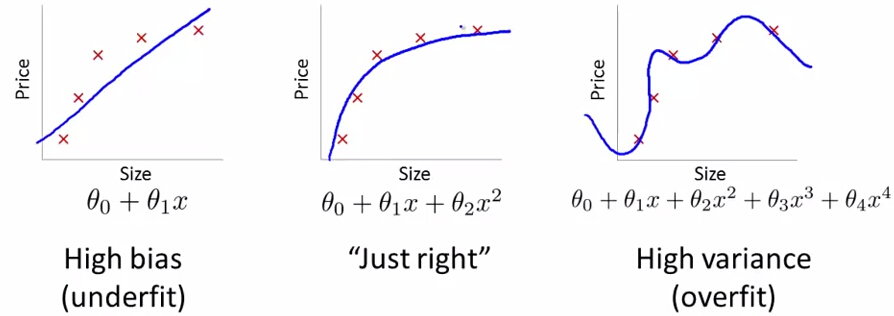
\includegraphics{picture/overfit.jpg}\textbackslash{}图10.过拟合

\paragraph{加入范数惩罚}\label{ux52a0ux5165ux8303ux6570ux60e9ux7f5a}

而常用的正规化的方法是直接将所有参数 (θ)
按某种形式加到最小化目标函数中加以惩罚,以免参数过大导致过拟合现象的产生,比如计算出来参数的
L1、L2范数然后直接把这一项加入到需要被优化的目标函数里去: {[}w = arg
min\_m\sum L(y\_i,f(x\_i;w))+\lambda \Omega(w){]}\textbackslash{}一般来说,监督训练可以看作是最小化上面的目标函数,而里面的
(L(y\_i,f(x\_i;w))) 是样本的预测的误差,后面的 (\Omega(w))
就是我加入的可以用来使模型更简单的正规化函数,比如L1范数正规化的话,有:
{[}\Omega(w) = \textbar{}\textbar{}w\textbar{}\textbar{}\_1 =
\sum\textbar{}w\_i\textbar{}{]}\textbackslash{}使用 L1
范数的正规化的话,还可以实现特征的稀疏表达。\textbackslash{}这个方法里的
(\lambda) 需要通过人工设定,可以通过实验来进行选择。

\paragraph{Max-norm}\label{max-norm}

除了上述的,通过在优化的目标函数里加入权值的范数来进行整个权值空间的惩罚以外,一种有效的正规化方法是
Max-norm。这种算法是在每个单个的隐藏单元里设置这个单元的传入的权值的 L2
范数的上限,如果权值的更新违反了这个约束,我就可以通过让这些权值除以这个范数来达到让这个权值重新正规化的目的。使用这个约束而不是使用惩罚的方法可以在无论每次权值更新得有多大的情况下防止权值变得非常大。而且,比起惩罚方法,使用约束的时候也可以使一开始的训练率可以取得很大,使得对权值空间的搜索可以更快,更彻底。当然,在这个算法里也有需要人工设置的参数,就是所使用的
L2 范数的上限。

\paragraph{Dropout}\label{dropout}

正规化的方法中,也有上述方法的变形。比如在网络的训练过程中使用的
Dropout\{{[}\}34\{{]}\}\{{[}\}35\{{]}\}算法。可以有效地加强模型的泛化能力,抑制神经网络出现过拟合的现象。\textbackslash{}Dropout
是指在模型训练时随机让网络某些隐含层节点的权值不工作,不工作的那些节点可以暂时认为不是网络结构的一部分,但是它的权值得保留下来(只是暂时这一轮里面它的值不更新而已),下次样本输入时它可能又会恢复工作了。但是这种方法是只适合于训练样本较少的条件下的用来增强模型的泛化能力的。\textbackslash{}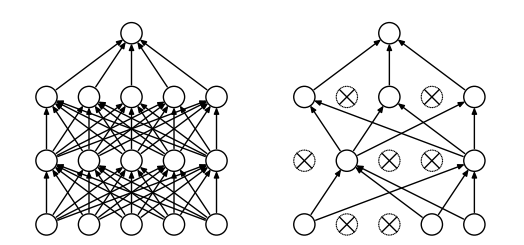
\includegraphics{picture/dropout.png}\textbackslash{}图11.左:标准神经网络;右:使用了
Dropout
算法之后\textbackslash{}而这个算法里需要人工调整的是让某些节点权值不工作的概率,一般会直接选择
50\%。

\subsubsection{Maxout}\label{maxout}

Maxout \{{[}\}36\{{]}\}
模型是类似多层感知机、卷积神经网络这种简单的前馈的架构使用的新型的激活函数。对于给定的输入
(x ∈ \Re)(x 可能是输入层的 (v) 或者是某一个隐含层的状态),通过一个
Maxout 自己的隐含层 (z),线性映射到输出的一个节点 (h(x)),连接的权值是
(W,b)。使用 Maxout
函数来作为激活函数可以加强模型对非线性函数的拟合能力,因为 Maxout
的拟合能力是非常强的,它可以拟合任意的的凸函数。最直观的解释就是任意的凸函数都可以由分段线性函数以任意精度拟合,而
Maxout 又是取k个自己的隐含层节点 (z) 的最大值,这些隐含层 (z)
节点也是线性的,所以在不同的取值范围下,最大值也可以看做是分段线性的(分段的个数与k值有关)。\textbackslash{}下图的例子表示
Maxout 可以拟合任意凸函数,当然也包括了ReLU(Rectifier
函数):\textbackslash{}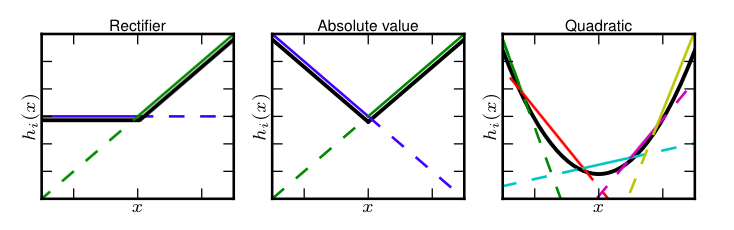
\includegraphics{picture/maxout.png}\textbackslash{}图12.Maxout可以拟合任意凸函数\textbackslash{}而
Maxout
拓扑关系如下图所示:\textbackslash{}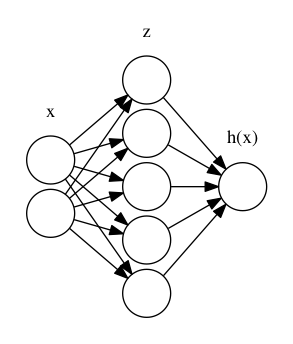
\includegraphics{picture/maxout-implement.png}\textbackslash{}图13.Maxout网络拓扑关系\textbackslash{}它的数学表达如下:\textbackslash{}{[}h(x)
= \{max\}\limits\emph{\{i∈{[}1,k{]}\}z}\{i\}{]} {[}z = x\^{}TW + b{]}
关于 Maxout 对凸函数的表达能力的证明,可以见\{{[}\}37\{{]}\}。

\subsection{框架选择}\label{ux6846ux67b6ux9009ux62e9}

本文中描述的算法,需要使用梯度下降的算法进行模型的优化。而建立出来的模型比如多层的神经网络,需要使用后向传播的算法,通过链式求导来得到各层链接的参数的导数。这里面有两个比较难以解决的问题:\textbackslash{}1.模型变得庞大之后,需要进行优化的参数的数量也会变得很大,计算耗费的时间非常多。\textbackslash{}2.导数计算的复杂程度会随网络层数的增加,还有网路里使用的算法的变化而变得越来越复杂;\textbackslash{}第一点可以用深度训练里的相关内容,比如自编码器里的逐层训练,还有有减少训练参数的特性的卷积神经网络来减缓。但是也不能解决这个问题,所以,需要有一个能够支持高性能的计算的平台来减少做计算实验的时间,加快模型的迭代和设计。目前的高性能的计算平台主要依靠分布式的计算机集群还有
GPU
进行计算。而目前对于我而言,最容易获得的高性能计算平台是基于高性能显卡的
GPU 计算平台。而要在编程的时候使用到 GPU
来进行算法的加速,就需要花精力训练相关的编程架构的知识,比如 NVIDIA 的
CUDA
框架。\textbackslash{}而第二点则可以通过编程来实现一些自动进行函数的求导之类的功能来辅助进行网络的设计,从而把研究者的精力从细节里解放出来,投入到模型的设计上去。但是如果让程序要能够设计复杂的计算过程,就需要有类似惰性求值的机制来把具体的计算推迟,让程序能够在不用计算出来具体的值,而是在开始计算之前的过程就能得到计算过程的式子的信息来进行其他的操作,比如通过知道代价函数的构造对权值求导。\textbackslash{}两点都是为了更好地去实验、设计模型。\textbackslash{}常用的进行机器训练使用的框架,有
Theano,Torch7,MATLAB 等。MATLAB
在使用小规模的数据进行验证的算法设计和实验的时候非常合适,可是当数据量变大后,要使用
GPU
去加速计算会比较麻烦,而且当模型变复杂之后,就要花时间去自行对模型中的参数进行求导。所以,我在做实验的时候优先选择使用
GPU
方便而且能够方便进行求导等高阶操作或者现成的资源比较丰富的框架。\textbackslash{}这两个框架各有千秋,鉴于
Theano 是使用 python
实现的,现成的语言和工具会比较丰富,所以,最后我选择的是 Theano
框架。\textbackslash{}下面,我就对两个比较常用的计算框架 Torch7 和
Theano
进行了简单的比较:\textbackslash{}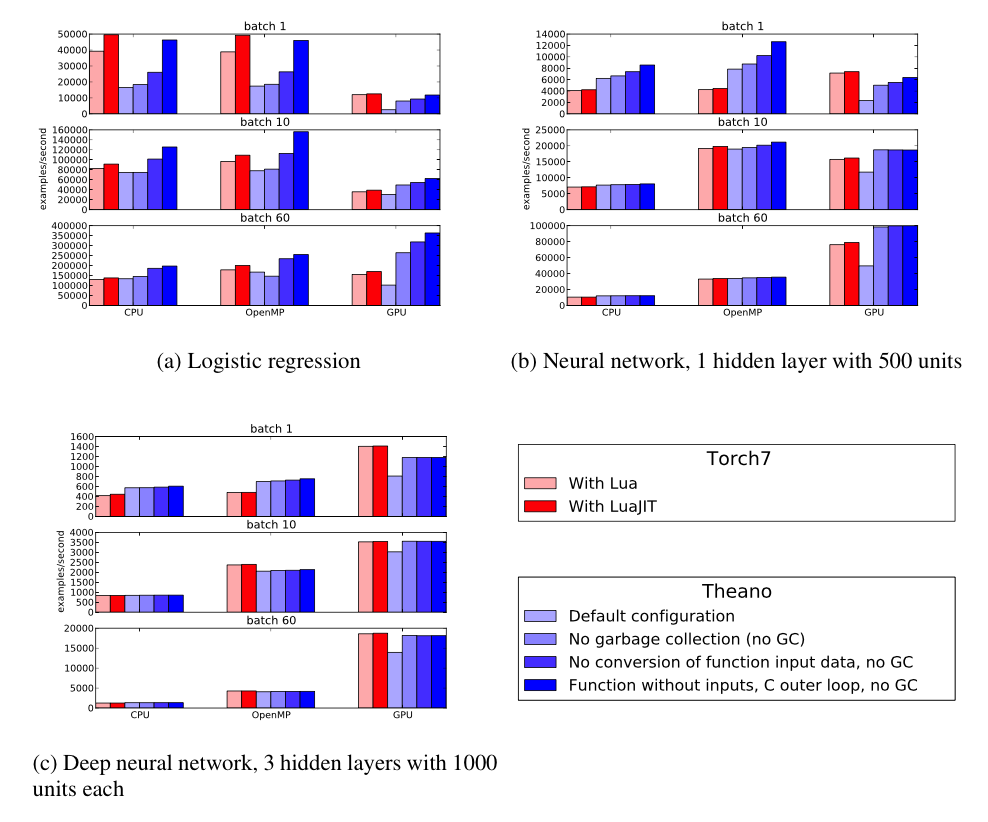
\includegraphics{picture/torch-vs-theano-speed.png}\textbackslash{}图14.Torch7
与 Theano 性能比较

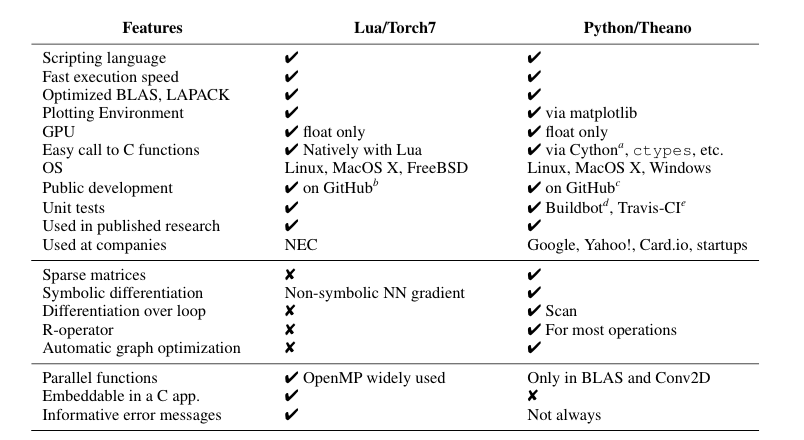
\includegraphics{picture/torch-vs-theano-feature.png}\textbackslash{}图15.Torch7
与 Theano 特性比较

\subsection{数据集}\label{ux6570ux636eux96c6}

本文中,用来作为标准并且进行试验的数据集是康奈尔大学的 CAD-60
数据集,这个数据集是用微软的 Kinect 传感器拍摄下来的,由人做特定的动作的
RGB-D
视频序列构成。而且数据集里还有预先获取到的人的骨架模型,本文中的我的实验就是基于数据集里的骨架模型的序列。\textbackslash{}CAD-60这个数据集有如下特点:
1.60个RGB-D的视频;\textbackslash{}2.4个对象:两男、两女;\textbackslash{}3.5个不同的环境:办公室、厨房、我是、浴室和起居室;\textbackslash{}4.12种活动:漱口、刷牙、戴隐形眼镜、谈电话、喝水、开药丸盒子、烹饪(切菜)、烹饪(搅拌),在沙发上聊天,在沙发上放松,在白板上写东西,在电脑前工作。\textbackslash{}这个骨架模型的描述方式如下图所示:\textbackslash{}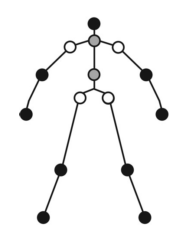
\includegraphics{picture/skeleton.png}\textbackslash{}图16.CAD-60骨架数据\{{[}\}11\{{]}\}\textbackslash{}数据集中的人物骨架是从
Kinect
的采集程序里直接获取,它们的排列是和视频里的每一个帧一一对应的。骨架中一共有
15 个关节的三维空间坐标,坐标是以 Kinect
摄像头为坐标系零点的绝对三维坐标值,其中 11
个关节有它所对应的关节的转向角的 (3*3)
的矩阵。所以,如果把每一帧中的骨架的信息当作一个数据点的话,每个点的数据的数量为
144 个,而且都是 32
位的浮点数,同时,我使用普通的线性变换吧所有的点的所有数值都做了一次归一化,以保证后面训练算法的有效:\textbackslash{}{[}
x\_\{norm\} = (x-min(x))/(max(x)-min(x)) ){]}。

数据集里,每个人的每个动作对应一个完整的视频(骨架)序列,长度在几十秒左右。\textbackslash{}为了让训练和测试的数据集更多,我把每一个长度达二、三千帧的序列按每
48
帧一组进行了切片并打标签的操作。并且按照取其中三个人作为训练集,第四个人作为测试集的方式分成了两大组数据。这样子处理完之后,我得到了一个大的数据集,数据集中的每个样本都是二维的
(144*48) 的数据。

\subsection{实验模型}\label{ux5b9eux9a8cux6a21ux578b}

我这次的实验主要尝试了两种模型,自编码器和卷积神经网络,并且在网络里使用了几种不同的能增强分类效果和模型泛化能力的技巧。下面会详细描述每个实验中的模型的设计。所有实验都是以三个人的运动为训练集,第四个人的运动为测试集的,通过训练已知的人运动去识别未知的人的运动可以有效检验模型的提取一般特征的泛化能力。所有模型在训练时,我都把样本先按顺序分成一批批(batch)
,然后 batch 之间再打乱顺序,一个个的 batch 放进去模型里进行训练。以
batch 进行训练的可以有效利用 GPU
,因为如果要一个个样本地放进模型里训练, CPU 和 GPU
之间要切换得很频繁,就没有办法发挥 GPU
的加速作用了。而打乱顺序是为了避免让模型陷入局部的解里,从而让模型能够得到一个更好的结果。

\subsubsection{5层的多层感知机}\label{ux5c42ux7684ux591aux5c42ux611fux77e5ux673a}

第一个要实验的是直接对原始数据使用普通的多层感知机作为分类器进行分类,而不是先使用其他的的特征提取的方法来进行训练、提取特征。而由于后面的模型里也是会使用多层的感知机作为分类器。由于普通的神经网络里的每一层都是一维的结构,所以原本的输入的
144*48
的这个二维的结构需要展开铺平成一维的结构,但是原来的数据的空间维度的信息就丢失了。这个多层感知机的设计如下图所示:\textbackslash{}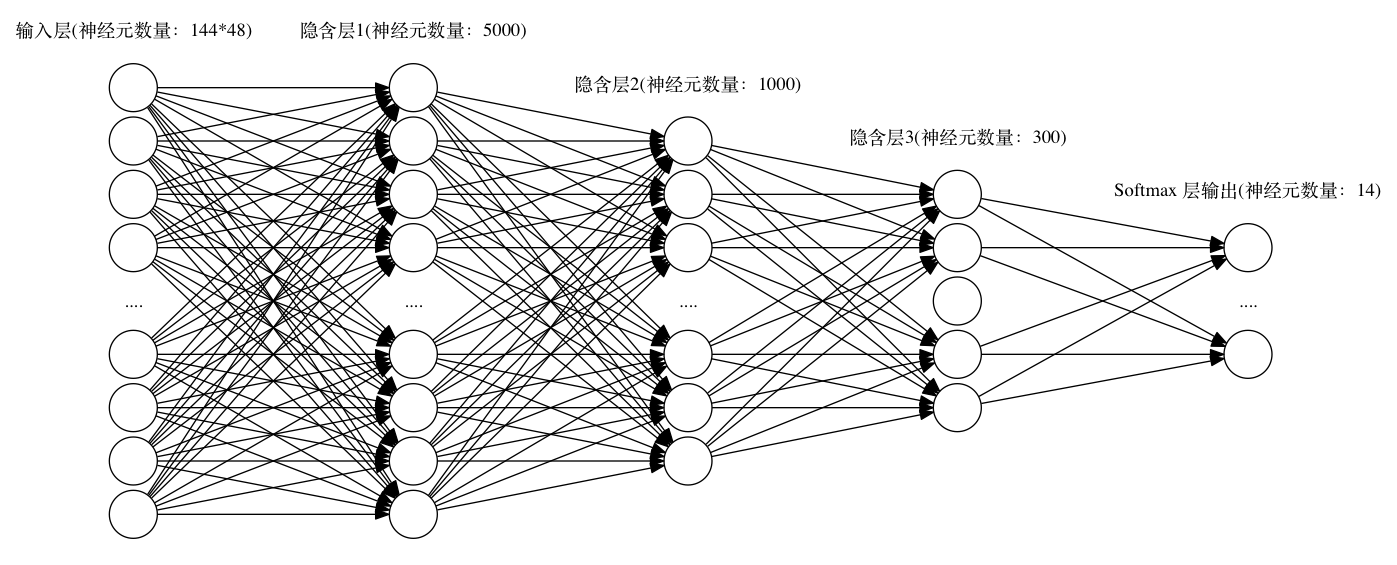
\includegraphics{picture/5l-mlp.png}\textbackslash{}图17.多层感知机分类器\textbackslash{}这个网络里面的激活函数使用的是
Sigmoid
函数。\textbackslash{}这里使用的这个模型的主要原因是为了给后面的模型的分类结果提供一个对照的基础,以表现这些特征提取的方法的效果,因此,在理解后面的模型的时候,可以把当前这个网络里的第一个隐含层替换为后面的模型的特征提取层,比如卷积网络或者自编码器。\textbackslash{}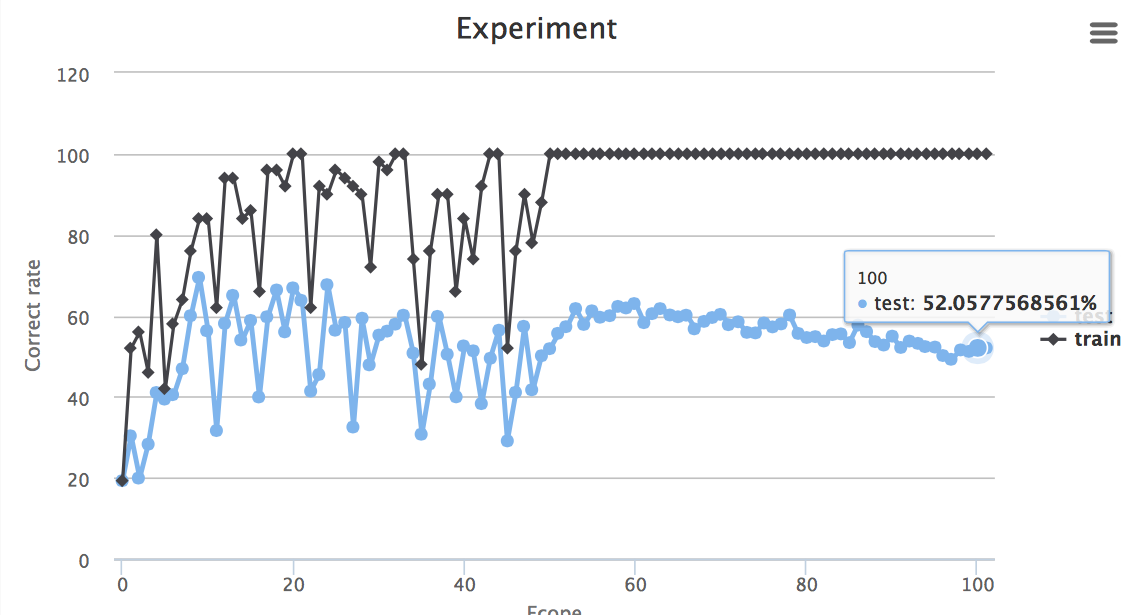
\includegraphics{picture/5l-mlp-experiment.png}\textbackslash{}图18.多层感知机实验结果\textbackslash{}上图中的横坐标是训练的代数(ecope),
所有来自训练集的各个 batch
的数据全进入模型训练完一次算是一代。而图中的纵坐标则是训练的正确率,每一次训练完一代的数据都把测试集的数据放进模型分类一次,然后看分类的正确率。

\subsubsection{自编码器+多层感知机}\label{ux81eaux7f16ux7801ux5668ux591aux5c42ux611fux77e5ux673a}

使用单层的自编码器代替多层感知机的第一层隐含层。先进行无监督学习来进行降维,然后再通过后面的多层感知机进行有监督的学习来进行分类。同样的,也需要跟上一个模型一样,需要把二维的输入的数据铺平到一维。但是由于无监督学习的时候没有加入标签的信息,而整个模型的层数和上一个模型的层数是差不多的,所以直觉上,这个模型的表达能力是会比上一个模型要弱的,具体的模型如下图所示:\textbackslash{}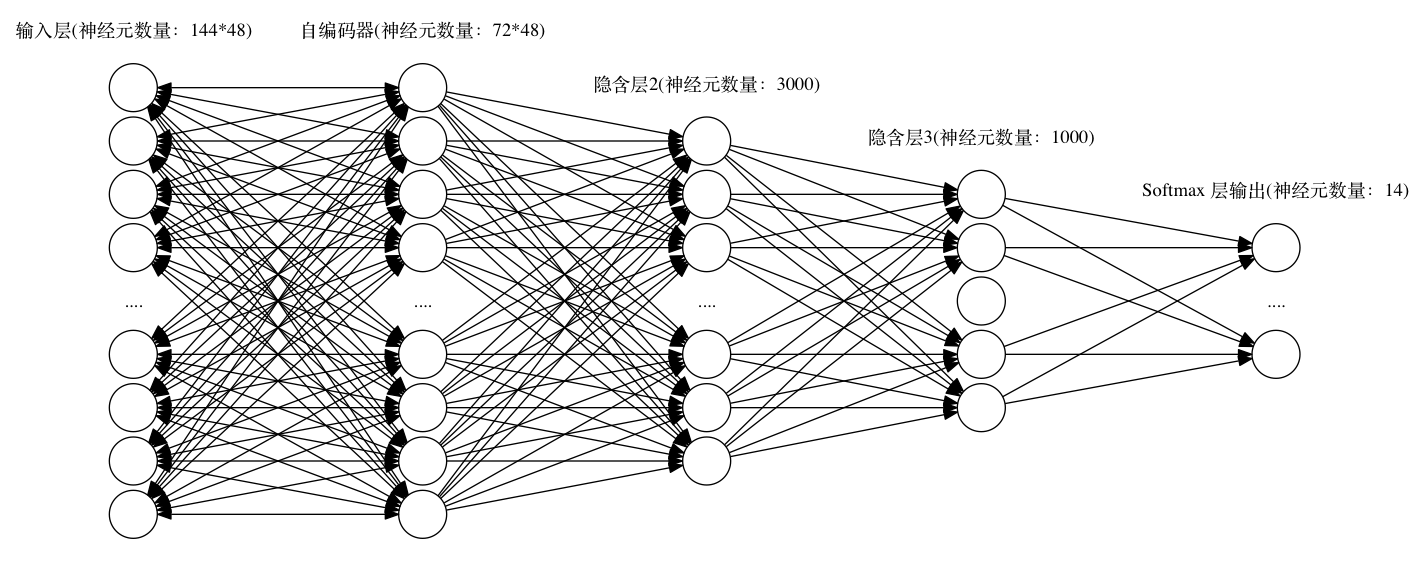
\includegraphics{picture/dac-mlp.png}\textbackslash{}图19.自编码器+多层感知机\textbackslash{}而这个模型的训练结果则如下图所示:\textbackslash{}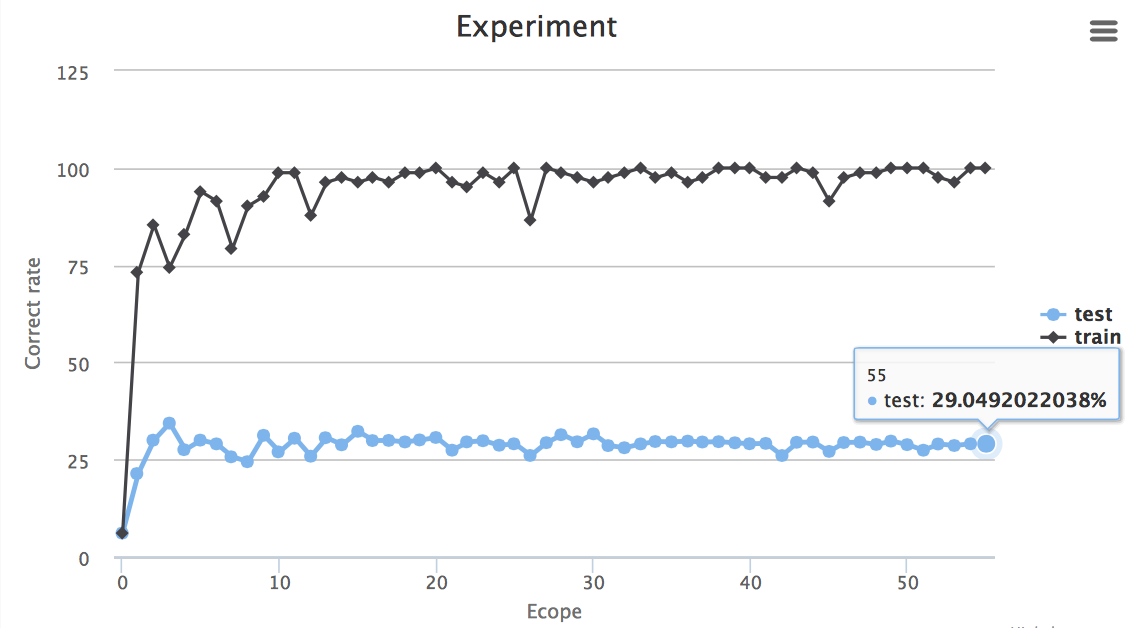
\includegraphics{picture/1dac-1mlp-experiment.png}\textbackslash{}图20.自编码器+多层感知机实验结果\textbackslash{}这个实验结果确实比上一个模型的要差很多。可能就是因为模型的表达能力比较弱的原因。于是后面的我又多加了一层自编码器在原来的自编码器后面,训练出来的结果是网络是发散的,分类结果是随机的,可能对于这个数据,使用自编码器来进行预训练会不合适。

\subsubsection{卷积神经网络+多层感知机}\label{ux5377ux79efux795eux7ecfux7f51ux7edcux591aux5c42ux611fux77e5ux673a}

由于卷积神经网络的输入就是需要经过二维卷积核进行卷积的,所以原来的二维结构的数据不需要进行铺平操作,直接以二维的模式进入网络进行学习就可以了。而且,由于这个数据的其中一个维度是时间,所以使用这个卷积网络还可以同时把时间维度的信息也考虑进来,使得整个模型能够更好地对时间维度的信息进行建模。由后面的多层感知机的输入神经元的大小可以看出来,原数据提取完特征之后只有
320
个变量,大大减轻了后面的分类器的计算压力。实验结果如下:\textbackslash{}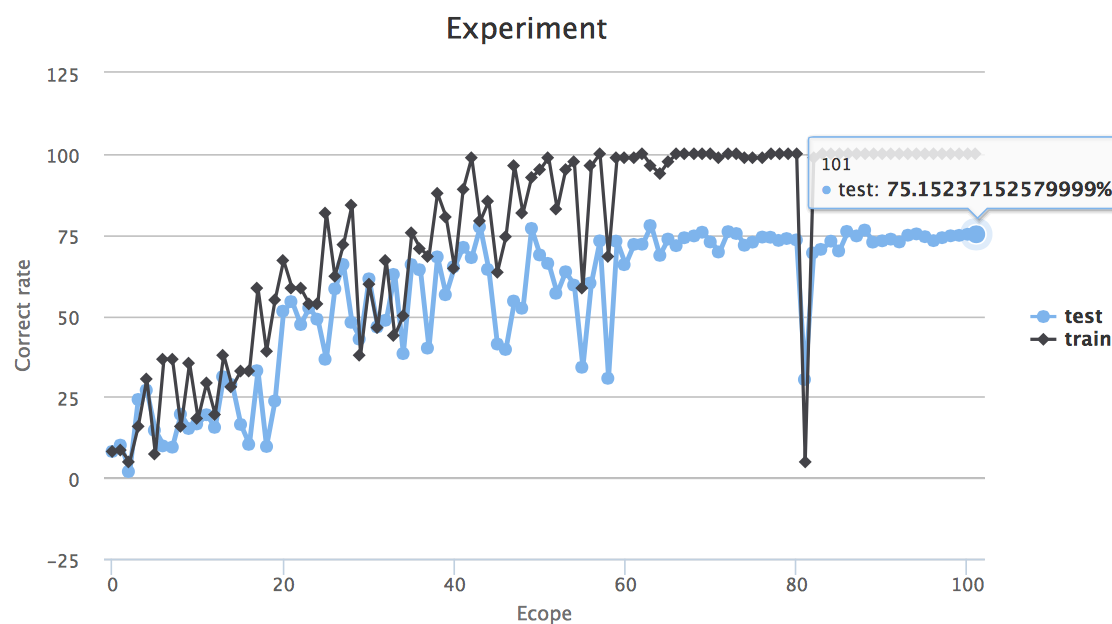
\includegraphics{picture/cnn-mlp-experiment.png}\textbackslash{}图21.卷积神经网络+多层感知机实验结果\textbackslash{}从上面的模型到现在这个的实验结果可以看出来,训练集的准确率已经接近
100\%
,但是测试集的准确率还是不高。显然模型的训练出现了过拟合的现象。所以接下来要做的事情应该是加强模型的泛化能力,阻止模型出现过拟合的现象。\textbackslash{}网络的结构如下图所示:\textbackslash{}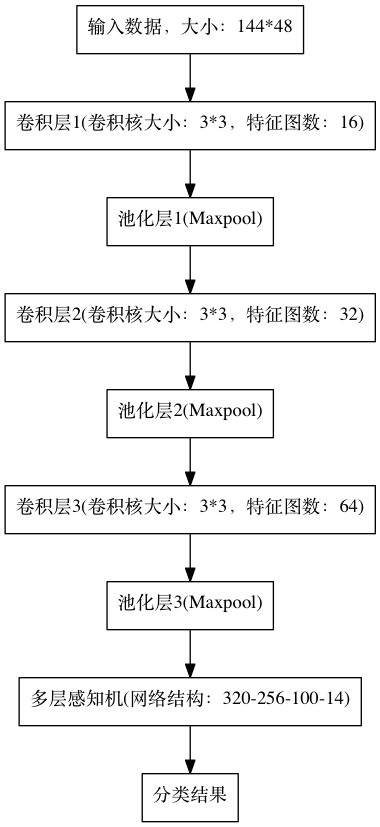
\includegraphics{picture/cnn-mlp.png}\textbackslash{}图22.卷积神经网络+多层感知机模型结构

\paragraph{加入正规化环节}\label{ux52a0ux5165ux6b63ux89c4ux5316ux73afux8282}

为了加快模型的收敛,我没有使用常规的在代价函数里加入惩罚环节来加强模型的泛化能力。而是使用了
Max-Norm 算法来对过大的权值进行惩罚。也就是把
L2范数超过一定阈值的神经元的权值除以范数来抑制它变得过大。加入了这个环节的模型的训练结果如下:\textbackslash{}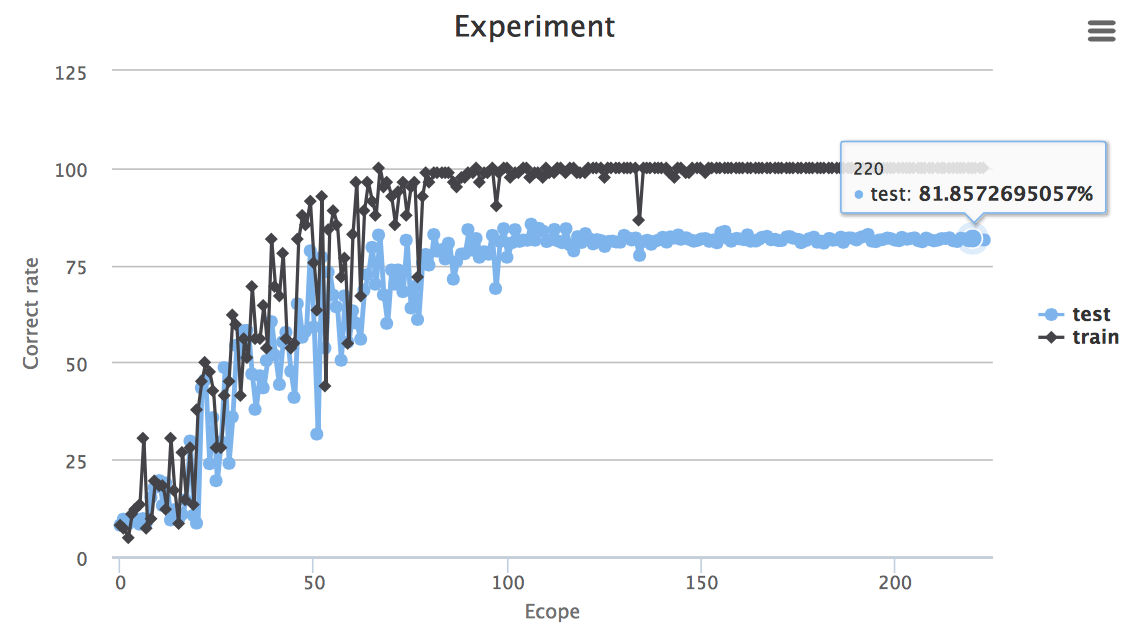
\includegraphics{picture/cnn-mlp-experiment-max-norm.png}\textbackslash{}图23.卷积神经网络+多层感知机模型加入正规化环节后实验结果\textbackslash{}可以看出来,加入了正规化环节之后,模型训练的时间变长了,而且训练数据集的训练识别率也更难达到
100\%
了。但是,相对的,测试数据集的识别率提高了不少,说明正规化环节对于抑制过耦合非常的有效。

\subsection{实验结果分析}\label{ux5b9eux9a8cux7ed3ux679cux5206ux6790}

\subsubsection{实验模型结果对比分析}\label{ux5b9eux9a8cux6a21ux578bux7ed3ux679cux5bf9ux6bd4ux5206ux6790}

由上面的各个实验可以看出来,结果最好的模型是加入了正规化环节的卷积神经网络+多层感知机。而另一个深度学习的算法------自编码器不太适用于当前的数据集,可能是因为这个自编码器的算法的对于时序数据的提取特征的能力不是太强,需要用一些方法去加强这个自编码器算法对于时序数据的处理能力。比如加入一些用来加强前后神经元相关性计算能力的环节。

\subsubsection{同行结果对比分析}\label{ux540cux884cux7ed3ux679cux5bf9ux6bd4ux5206ux6790}

下表为针对 CAD-60 数据集的同行论文的结果。

\begin{longtable}[c]{@{}lcl@{}}
\caption{同行算法准确率对比表}\tabularnewline
\toprule
& New Person &\tabularnewline
\midrule
\endfirsthead
\toprule
& New Person &\tabularnewline
\midrule
\endhead
Algorithm & Precision (\%) & Recall (\%)\tabularnewline
Shan, Akella, ARSO 2014 {[}19{]} & 93.8 & 94.5\tabularnewline
Zhu, Chen, Guo, IVC 2014 {[}9{]} & 93.2 & 84.6\tabularnewline
Parisi, Weber, Wermter, Front. Neurobot. 2015 {[}38{]} & 91.9 &
90.2\tabularnewline
Faria, Premebida, Nunes, RO-MAN 2014 {[}18{]} & 91.1 &
91.9\tabularnewline
Zhang, Tian, NWPJ 2012 {[}39{]} & 86 & 84\tabularnewline
本文 & 81.8 & -\tabularnewline
Koppula, Gupta, Saxena, IJRR 2012. {[}40{]} & 80.8 & 71.4\tabularnewline
Gupta, Chia, Rajan, MM 2013 {[}41{]} & 78.1 & 75.4\tabularnewline
Gaglio, Lo Re, Morana, HMS 2014 {[}11{]} & 77.3 & 76.7\tabularnewline
Ni et al., Cybernetics 2013 {[}14{]} & 75.9 & 69.5\tabularnewline
Wang et al., PAMI 2013 {[}42{]} & 74.7 & -\tabularnewline
Yang, Tian, JVCIR 2013 {[}16{]} & 71.9 & 66.6\tabularnewline
Piyathilaka, Kodagoda, ICIEA 2013 {[}38{]} & 70 & 78\tabularnewline
Sung et al., AAAI PAIR 2011, ICRA 2012. {[}22{]} & 67.9 &
55.5\tabularnewline
Ni, Moulin, Yan, ECCV 2012 {[}43{]} & 65.32 & -\tabularnewline
\bottomrule
\end{longtable}

上表中的一些论文是使用精确率(Precision)和召回率(Recall)来描述其结果的,另外的是与本文一样直接用准确率(Accuracy)作为实验结果的。\textbackslash{}这三个评估标准的定义如下:

\begin{longtable}[c]{@{}lcc@{}}
\caption{样本分类类型定义}\tabularnewline
\toprule
& 相关,正类 & 无关,负类\tabularnewline
\midrule
\endfirsthead
\toprule
& 相关,正类 & 无关,负类\tabularnewline
\midrule
\endhead
被检索到 & TP & FP\tabularnewline
未被检索到 & FN & TN\tabularnewline
\bottomrule
\end{longtable}

Precision: {[}P=\frac{TP}{TP+FP}{]} Recall: {[}R=\frac{TP}{TP+FN}{]}
Accuracy: {[}A=\frac{TP+TN}{TP+FP+FN+TN}{]}

\section{总结与展望}\label{ux603bux7ed3ux4e0eux5c55ux671b}

\subsection{总结}\label{ux603bux7ed3}

本文先是总结了现有的人体运动类型识别的算法的普遍框架:人工提取特征然后再使用分类器进行分类。提出了使用深度学习理论进行自动的特征提取,并且使用深度学习里面的自编码器和卷积神经网络进行自动的特征提取。并且给出了相应的实验结果,最终得到了一个有着不错效果的,人体运动类型识别的模型------卷积神经网络+多层感知机。

\subsection{展望}\label{ux5c55ux671b}

\subsubsection{加入提前停止法}\label{ux52a0ux5165ux63d0ux524dux505cux6b62ux6cd5}

由各个训练实验的结果的曲线来看,在使用训练的数据集训练到训练的准确率达到
100\%
之后,测试集的测试的准确率也往往到达了最大值,往后面就开始以缓慢的速度下降。由此可见,在训练集的准确率达到
100\%
之后模型再训练下去,泛化能力反而会下降,逐渐出现过拟合的现象。所以还应该在训练的算法里加入提前停止的环节,也就是提前停止法,具体的,可以根据\{{[}\}44\{{]}\}展开研究。

\subsubsection{更换其他分类器}\label{ux66f4ux6362ux5176ux4ed6ux5206ux7c7bux5668}

由实验可以看到卷积神经网络具有非常优良的提取特征的能力,能够提高分类模型的分类能力。而在论文里就有不少使用
SVM、朴素贝叶斯等经典的分类器取得非常好的分类结果的模型。而且,使用有效的特征提取算法也可以减少像
SVM
这样子的算法训练的时候所需要的时间。所以,可以综合卷积神经网络的特征提取能力和其他分类器的分类能力去创造新的模型。而综合两者有两种思路,一种是通过把后向传播算法推广到其他的分类器,使得可以直接使用这些分类器去传播误差,从而训练要使用得到的卷积神经网路。另一种思路是使用浅层的使用ReLU激活函数的神经网络,直接使用有监督学习对卷积神经网路进行训练。之所以使用浅层的神经网络是因为可以一来减少后面的网络结构对卷积神经网络的训练的影响,二来可以减少误差传递过程中的损失,避免误差传递到卷积神经网络的表层时已经变得很小,从而影响卷积神经网络的训练。而所说的这两种方法都需要做实验去确定效果和是否行得通。

\section{致谢}\label{ux81f4ux8c22}

感谢莫凌飞老师还有邵思羽学姐在论文撰写期间提供的帮助和指导。感谢我看的论文的作者们,你们的努力工作和聪明才智还有发表论文时的不厌其烦都极大地启发了我的思路。感谢空空如也的钱包,让我在论文的写作期间完全没有别的杂念。感谢在我通宵工作时没有因为我敲键盘声音太大而弄死我的室友。感谢陈琦同学提供的帮助,如果没有他的帮助,我可以提前一个月完成这篇论文。

\section*{引用文献}\label{ux5f15ux7528ux6587ux732e}\addcontentsline{toc}{section}{引用文献}

\{{[}\}1\{{]}\}L. Chen, H. Wei, and J. Ferryman, ``A survey of human
motion analysis using depth imagery,''
\emph{Pattern Recognition Letters}, vol.~34, no. 15, pp.~1995--2006,
2013.

\{{[}\}2\{{]}\}D. Weinland, M. Özuysal, and P. Fua, ``Making action
recognition robust to occlusions and viewpoint changes,'' in
\emph{Lecture notes in
computer science (including subseries lecture notes in artificial
intelligence and lecture notes in bioinformatics)}, 2010, vol.~6313
LNCS, pp.~635--648.

\{{[}\}3\{{]}\}L.-c. Chen, J.-w. Hsieh, C.-h. Chuang, C.-y. Huang, and
D. Y. Chen, ``Occluded Human Action Analysis Using Dynamic Manifold
Model,'' in \emph{International conference on pattern recognition},
2012, pp.~1245--1248.

\{{[}\}4\{{]}\}M. B. Holte, T. B. Moeslund, N. Nikolaidis, and I. Pitas,
``3D Human Action Recognition for Multi-view Camera Systems,'' in
\emph{2011
international conference on 3D imaging, modeling, processing,
visualization and transmission}, 2011, pp.~342--349.

\{{[}\}5\{{]}\}D. Weinland, E. Boyer, and R. Ronfard, ``Action
recognition from arbitrary views using 3D exemplars,'' in
\emph{Proceedings of the iEEE
international conference on computer vision}, 2007, pp.~1--7.

\{{[}\}6\{{]}\}M. C. Roh, H. K. Shin, and S. W. Lee, ``View-independent
human action recognition with Volume Motion Template on single stereo
camera,'' \emph{Pattern Recognition Letters}, vol.~31, no. 7,
pp.~639--647, 2010.

\{{[}\}7\{{]}\}M.-y. Chen, ``MoSIFT : Recognizing Human Actions in
Surveillance Videos MoSIFT : Recognizing Human Actions in Surveillance
Videos.'' 2009.

\{{[}\}8\{{]}\}R. Poppe, ``A survey on vision-based human action
recognition,'' \emph{Image and Vision Computing}, vol.~28, no. 6,
pp.~976--990, 2010.

\{{[}\}9\{{]}\}Y. Zhu, W. Chen, and G. Guo, ``Evaluating spatiotemporal
interest point features for depth-based action recognition,''
\emph{Image and
Vision Computing}, vol.~32, no. 8, pp.~453--464, 2014.

\{{[}\}10\{{]}\}L. Piyathilaka and S. Kodagoda, ``Gaussian mixture based
HMM for human daily activity recognition using 3D skeleton features,''
\emph{Proceedings of the 2013 IEEE 8th Conference on Industrial
Electronics and Applications, ICIEA 2013}, pp.~567--572, 2013.

\{{[}\}11\{{]}\}S. Gaglio, G. L. Re, S. Member, and M. Morana, ``Human
Activity Recognition Process Using 3-D Posture Data,'' pp.~1--12, 2014.

\{{[}\}12\{{]}\}L. Rybok, B. Schauerte, Z. Al-Halah, and R.
Stiefelhagen, ```Important stuff, everywhere!`Activity recognition with
salient proto-objects as context,'' \emph{2014 IEEE Winter Conference on
Applications of Computer Vision, WACV 2014}, pp.~646--651, 2014.

\{{[}\}13\{{]}\}N. Dalal and B. Triggs, ``Histograms of oriented
gradients for human detection,'' in
\emph{Proceedings - 2005 iEEE computer society
conference on computer vision and pattern recognition, cVPR 2005}, 2005,
vol.~I, pp.~886--893.

\{{[}\}14\{{]}\}B. Ni, Y. Pei, P. Moulin, and S. Yan, ``Multilevel depth
and image fusion for human activity detection,''
\emph{IEEE Transactions on
Cybernetics}, vol.~43, no. 5, pp.~1382--1394, 2013.

\{{[}\}15\{{]}\}R. Chaudhry, a. Ravichandran, G. Hager, and R. Vidal,
``Histograms of oriented optical flow and Binet-Cauchy kernels on
nonlinear dynamical systems for the recognition of human actions,''
\emph{2009 IEEE Conference on Computer Vision and Pattern Recognition},
pp.~1932--1939, 2009.

\{{[}\}16\{{]}\}X. Yang and Y. Tian, ``Effective 3D action recognition
using EigenJoints,'' \emph{Journal of Visual Communication and Image
Representation}, vol.~25, no. 1, pp.~2--11, 2014.

\{{[}\}17\{{]}\}K. Lertniphonphan, S. Aramvith, and T. H.
Chalidabhongse, ``Human action recognition using direction histograms of
optical flow,''
\emph{2011 11th International Symposium on Communications \& Information
Technologies (ISCIT)}, vol.~c, no. Iscit, pp.~574--579, 2011.

\{{[}\}18\{{]}\}D. R. Faria, C. Premebida, and U. Nunes, ``A
Probabilistic Approach for Human Everyday Activities Recognition using
Body Motion from RGB-D Images,''
\emph{IEEE International Symposium on Robot and
Human Interactive Communication (Ro-Man)}, 2014.

\{{[}\}19\{{]}\}J. Shan and S. Akella, ``3D Human Action Segmentation
and Recognition using Pose Kinetic Energy,'' 2014.

\{{[}\}20\{{]}\}N. Hu, G. Englebienne, Z. Lou, and B. Kr, ``Learning
Latent Structure for Activity Recognition *,'' pp.~1048--1053, 2014.

\{{[}\}21\{{]}\}C. Zhang and Y. Tian, ``RGB-D camera-based activity
analysis,''
\emph{\ldots{}and Conference (APSIPA ASC), 2012 Asia- \ldots{}}, 2012.

\{{[}\}22\{{]}\}J. Sung, C. Ponce, B. Selman, and A. Saxena, ``Human
Activity Detection from RGBD Images,'' 2011.

\{{[}\}23\{{]}\}I. Arel, D. C. Rose, and T. P. Karnowski, ``Deep Machine
Learning --- A New Frontier in Artificial Intelligence Research,''
\emph{IEEE Computational Inteligence Magazine}, vol.~5, no. 4,
pp.~13--18, 2010.

\{{[}\}24\{{]}\}R. E. Bellman,
\emph{Chapter 6 Dynamic programming algorithms}, vol.~11. 1987,
pp.~343--395.

\{{[}\}25\{{]}\}A. F. Marquand, S. \{De Simoni\}, O. G. O'Daly, S. C. R.
Williams, J. Mourão-Miranda, and M. a Mehta,
\emph{Pattern classification of
working memory networks reveals differential effects of methylphenidate,
atomoxetine, and placebo in healthy volunteers.}, vol.~36. 2011,
pp.~1237--1247.

\{{[}\}26\{{]}\}S. Wold, K. Esbensen, and P. Geladi, ``Principal
component analysis,''
\emph{Chemometrics and intelligent laboratory systems}, vol.~2.
pp.~37--52, 1987.

\{{[}\}27\{{]}\}K. Pearson, ``LIII. On lines and planes of closest fit
to systems of points in space,'' \emph{The London, Edinburgh, and Dublin
Philosophical Magazine and Journal of Science}, vol.~2, pp.~559--572,
1901.

\{{[}\}28\{{]}\}Y. Lecun, ``Deep Learning Tutorial,''
\emph{ICML2013 Tutorial}, 2013.

\{{[}\}29\{{]}\}Y. Bengio, ``Learning Deep Architectures for AI,''
\emph{Foundations and trends® in machine learning}, vol.~2. pp.~1--127,
2009.

\{{[}\}30\{{]}\}Y. LeCun, L. Bottou, Y. Bengio, and P. Haffner,
``Gradient-based learning applied to document recognition,''
\emph{Proceedings of the
IEEE}, vol.~86, no. 11, pp.~2278--2323, 1998.

\{{[}\}31\{{]}\}F. J. Huang and Y. LeCun, ``Large-scale learning with
SVM and convolutional nets for generic object categorization,'' in
\emph{Proceedings of the iEEE computer society conference on computer
vision and pattern recognition}, 2006, vol.~1, pp.~284--291.

\{{[}\}32\{{]}\}D. Kriesel,
\emph{A Brief Introduction to Neural Networks}. 2007.

\{{[}\}33\{{]}\}Y. A. LeCun, L. Bottou, G. B. Orr, and K. R. Müller,
``Efficient backprop,''
\emph{Lecture Notes in Computer Science (including subseries
Lecture Notes in Artificial Intelligence and Lecture Notes in
Bioinformatics)}, vol.~7700 LECTU, pp.~9--48, 2012.

\{{[}\}34\{{]}\}G. Hinton, ``Dropout : A Simple Way to Prevent Neural
Networks from Overfitting,''
\emph{Journal of Machine Learning Research (JMLR)}, vol.~15,
pp.~1929--1958, 2014.

\{{[}\}35\{{]}\}G. E. Hinton, N. Srivastava, A. Krizhevsky, I.
Sutskever, and R. R. Salakhutdinov, ``Improving neural networks by
preventing co-adaptation of feature detectors,''
\emph{arXiv: 1207.0580}, pp.~1--18, 2012.

\{{[}\}36\{{]}\}I. J. Goodfellow, D. Warde-Farley, M. Mirza, A.
Courville, and Y. Bengio, ``Maxout Networks,'' \emph{arXiv preprint},
pp.~1319--1327, 2013.

\{{[}\}37\{{]}\}S. Wang, ``General constructive representations for
continuous piecewise-linear functions,''
\emph{IEEE Transactions on Circuits and
Systems I: Regular Papers}, vol.~51, no. 9, pp.~1889--1896, 2004.

\{{[}\}38\{{]}\}G. I. Parisi, C. Weber, and S. Wermter,
``Self-Organizing Neural Integration of Pose-Motion Features for Human
Action Recognition,'' 2015.

\{{[}\}39\{{]}\}C. Zhang and Y. Tian, ``RGB-D Camera-based Daily Living
Activity Recognition,''
\emph{Journal of Computer Vision and Image Processing}, vol.~2, p.~12,
2012.

\{{[}\}40\{{]}\}H. S. Koppula, R. Gupta, and a. Saxena, ``Learning human
activities and object affordances from RGB-D videos,'' \emph{The
International Journal of Robotics Research}, vol.~32, no. 8,
pp.~951--970, 2013.

\{{[}\}41\{{]}\}R. Gupta, A. Y.-S. Chia, and D. Rajan, ``Human
activities recognition using depth images,''
\emph{Proceedings of the 21st ACM
international conference on Multimedia}, pp.~283--292, 2013.

\{{[}\}42\{{]}\}J. Wang, Z. Liu, Y. Wu, and J. Yuan, ``Learning
actionlet ensemble for 3D human action recognition,''
\emph{IEEE Transactions on
Pattern Analysis and Machine Intelligence}, vol.~36, no. 5,
pp.~914--927, 2014.

\{{[}\}43\{{]}\}B. Ni, P. Moulin, and S. Yan, ``LNCS 7573 -
Order-Preserving Sparse Coding for Sequence Classification,''
pp.~173--187, 2012.

\{{[}\}44\{{]}\}L. Prechelt, ``Early stopping - But when?''
\emph{Lecture Notes
in Computer Science (including subseries Lecture Notes in Artificial
Intelligence and Lecture Notes in Bioinformatics)}, vol.~7700 LECTURE
NO, pp.~53--67, 2012.
